\renewcommand{\figurename}{Rys.}

\chapter*{Wprowadzenie}
\label{cha:wprowadzenie}
\addcontentsline{toc}{chapter}{Wprowadzenie}

\section*{Podstawowe parametry życiowe}
\label{sec:ParametryZyciowe}
\addcontentsline{toc}{section}{Podstawowe parametry życiowe}

\fontsize{14}{15}\selectfont

Monitorowanie stanu pacjentów jest istotnym elementem opieki pielęgniarskiej i~anestezjologicznej, gdyż dostarcza podstawowych 
informacji na temat bieżącej kondycji organizmu. Rejestracja podstawowych parametrów ustroju jest prowadzona w~sposób ciągły 
na oddziałach intensywnej terapii, chirurgii, pediatrii i~podczas przeprowadzania prób wysiłkowych w~kardiologii oraz medycynie 
sportowej. Systematyczny monitoring wybranych parametrów, umożliwia natychmiastowe wykrycie odchyleń wskaźników od norm, co 
może być oznaką pogorszenia stanu zdrowia lub zagrożenia życia pacjenta. Parametry te to m.in.:

\begin{itemize}
	\item temperatura
	\item częstość akcji serca
	\item częstość oddechów
	\item ciśnienie tętnicze krwi
	\item wysycenie krwi tlenem.
\end{itemize}

Pomiar temperatury, dokonywany poprzez umieszczenie~w ustach, uchu lub dole pachowym termometru, pozwala na zidentyfikowanie gorączki, 
hipotermii (obniżenia temperatury ciała) oraz ich wykluczenie, poprzez stwierdzenie normy. W zależności od miejsca pomiaru temperatury 
otrzymuje się wartości, których średnia wynosi: 36,8\textdegree~C~\cite{SzGa11}.\\

Tętno, czyli częstość skurczów serca na minutę, to rytmiczne rozciąganie naczyń krwionośnych wywołane nagłymi zmianami ciśnienia krwi 
w~następstwie skurczów i~rozkurczów komór serca. Można je mierzyć palpacyjnie, poprzez uciśnięcie danej tętnicy i~liczenie ilości uderzeń 
fal tętna lub za pomocą urządzeń rejestrujących tętno z~elektrod EKG i~pulsoksymetru.
Częstotliwość tętna u~człowieka zależy od wieku, wysiłku fizycznego, stanów emocjonalnych, choroby. W~wieku dojrzałym wynosi średnio 72 
uderzenia na minutę, w~wieku starszym średnio 67~\cite{SzGa11}.\\

Proces wymiany gazowej ustroju polega na dostarczaniu komórkom tlenu i~wydalaniu na zewnątrz dwutlenku węgla. Częstotliwość oddechów to liczba 
uniesień klatki piersiowej w~ciągu określonego przedziału czasu, najczęściej 60 sekund.
Częstość oddychania u~ludzi zdrowych wynosi 16-18 razy na 1 minutę u~dorosłych, 20-30 razy u~dzieci, 30-35 u~noworodka~\cite{SzGa11}. W~warunkach 
fizjologicznych na zmianę szybkości oddychania wpływa wzmożony wysiłek fizyczny, stany emocjonalne. W~warunkach patologicznych na przyspieszenie 
oddychania wpływają: stany gorączkowe, bolesne urazy, zabiegi operacyjne.\\

Ciśnienie tętnicze to ciśnienie wywierane przez krew na ścianki tętnic, przy czym rozumie się pod tą nazwą ciśnienie w~największych tętnicach, 
np.~w~tętnicy w~ramieniu. W~momencie skurczu serca, kiedy porcja krwi wypychana jest z~serca do aorty, w~tętnicach panuje najwyższe ciśnienie, 
wynoszące zazwyczaj u~zdrowego dorosłego człowieka od ok. 90 do 135 mmHg. W~chwili rozkurczu wartość ciśnienia krwi jest najniższa, np.~od ok. 50 
do 90~mmHg~\cite{SzGa11}. Pomiarów zazwyczaj dokonuje się metodą Korotkowa, przy użyciu sfigmomanometru i~słuchawek lekarskich, bądź metodami półautomatycznymi.\\

Saturacja oznacza nasycenie cieczy gazem. W~medycynie dokonuje się pomiarów nasycenia płynów ustrojowych, m.in.~krwi czy płynu komórkowego, gazami.
Najbardziej powszechnym pomiarem saturacji w~działaniach medycznych jest pomiar nasycenia krwi tętniczej tlenem metodą pulsoksymetrii w~celu 
przeciwdziałania niewydolności oddechowej. Pomiar wyznacza stopień wiązania hemoglobiny we krwi z~tlenem (zawartości oksyhemoglobiny). Wartość 
saturacji krwi tlenem u zdrowych ludzi zawiera się w~zakresie SpO2 95\%~–~99\%~\cite{SzGa11}. Saturacja poniżej 90\% oznacza niedotlenienie, 
które może być spowodowane m.in. przez niedokrwistość (anemię).\\

Rozpoznawanie i~ocena zjawisk fizjologicznych i~patologicznych towarzyszących zabiegom operacyjnym i~terapeutycznym oraz procesom chorobowym wymagają 
ciągłego lub powtarzalnego w~określonych odstępach czasu monitorowania wszystkich podstawowych parametrów życiowych. W~skład standardowego 
stanowiska anestezjologicznego wchodzą urządzenia umożliwiające pomiar i~obrazowanie powyższych wskaźników zintegrowane w~centralny monitor 
pacjenta~(rys. \ref{rys:central_monitor}).
\begin{figure}[!h]
	\centerline{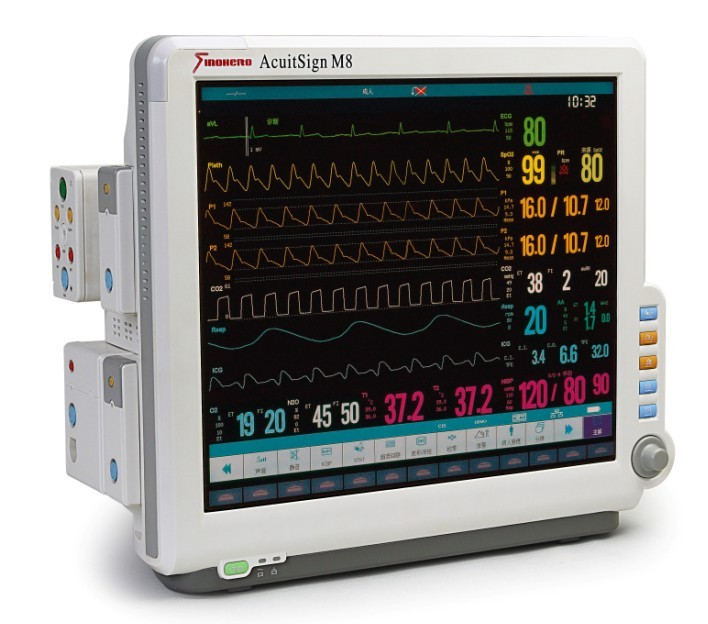
\includegraphics[scale = 0.45]{graphic/patient_monitor.jpg}}
	\caption{Centralny monitor pacjenta}
	~\\	 
	(źródło: http://www.axmeditec.com.pl)
	\label{rys:central_monitor}
\end{figure}

%---------------------------------------------------------------------------
\section*{Nieinwazyjne metody rejestracji sygnałów biomedycznych}
\label{sec:MetodyPomiarow}
\addcontentsline{toc}{section}{Nieinwazyjne metody rejestracji sygnałów biomedycznych.}

Istnieją różne sposoby ratowania i~ochrony życia. Aby określić najlepszą metodę leczenia pacjentów, specjaliści muszą wziąć pod uwagę różnorodne 
czynniki. Obok perspektywy medyczno-terapeutycznej dużą rolę odgrywa też fizyczna i~psychiczna presja wywierana na pacjenta podczas leczenia, 
jak również czas wymagany do zastosowania danego środka. Celem jest osiągnięcie jak najszybszego i~bezproblemowego procesu leczenia, przy czym 
ważną rolę odgrywają również aspekty ekonomiczne, które należy wziąć pod uwagę podczas wyboru odpowiedniej procedury diagnostycznej i~terapeutycznej. 
Zastosowanie nieinwazyjnych technologii może przyczynić się do zwiększenia dobrego samopoczucia pacjenta oraz uniknięcia powikłań podczas leczenia.

Nieinwazyjne metody monitorowania pacjenta są szybkie i~oszczędne. Ponadto są one najbardziej atrakcyjną alternatywą dla pacjentów i~mogą pomóc 
w~unikaniu infekcji. Przyczyną tego jest fakt, że każda ingerencja w~ciało, np. przy użyciu igieł lub cewników, otwiera szeroko drzwi infekcjom. 
W~sytuacji, która i~tak jest już stresująca dla pacjenta, pomiary inwazyjne zazwyczaj powodują dodatkowy ból i~stres.

Współczesne techniki obrazowania wykorzystują szereg zjawisk fizycznych umożliwiających nieinwazyjną rejestrację biosygnałów bez konieczności 
ingerencji chirurgicznej. Interakcja fali mechanicznej w~postaci ultradźwięków, pola magnetycznego oraz szerokiego zakresu promieniowania 
elektromagnetycznego~(rys. \ref{rys:spectrum}) z~ustrojem, stanowi bogate źródło użytecznych sygnałów, niosących istotne informacje na temat 
formy i~kondycji organizmu.
\begin{figure}[!h]
	\centerline{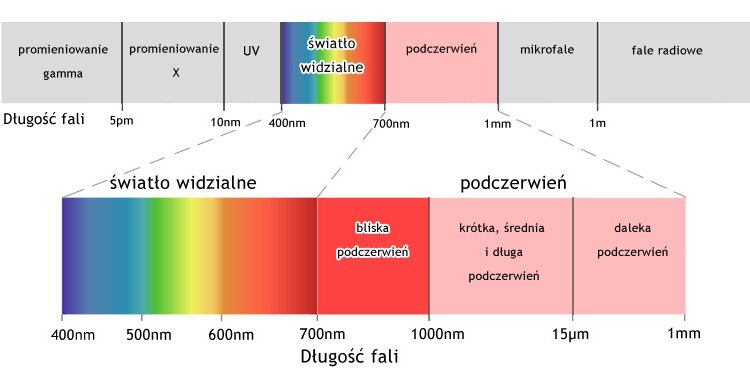
\includegraphics[scale = 0.56]{graphic/spectrum.jpg}}
	\caption{Spektrum fal elektromagnetycznych}
	~\\	
	(źródło: http://www.zebu.uoregon.edu)
	\label{rys:spectrum}
\end{figure}

\noindent Do najczęściej stosowanych metod obrazowania oraz diagnostyki w~praktyce medycznej należą~\cite{SzGa11}:
\begin{itemize}
	\item pulsoksymetria
	\item rentgenografia i~mammografia (RTG)
	\item ultrasonografia (USG)
	\item tomografia komputerowa (CT)
	\item tomografia rezonansu magnetycznego (MRT)
	\item pozytonowa tomografia emisyjna (PET)
	\item optyczna tomografia koherencyjna (OCT).\\
\end{itemize}

Wraz z~dynamicznym rozwojem technologii oraz tendencją do miniaturyzacji urządzeń i~przyrządów elektronicznych, pojawia się szereg nowych możliwości
i~perspektyw związanych z~obszarem obrazowania medycznego. Spośród różnorodnych usług realizowanych przez systemy telemedyczne, szczególnie istotną 
rolę odgrywa zdalne monitorowanie stanu pacjenta w~zakresie śledzenia wybranych parametrów i~sygnałów fizjologicznych. Temperatura, tętno, saturacja
czy ciśnienie krwi to wskaźniki, których wartości mogą być śledzone w~sposób ciągły w~trakcie wykonywania codziennych czynności i~podczas snu, nie 
wprowadzając dyskomfortu podczas ich rejestracji. 
%---------------------------------------------------------------------------

\section*{Cel i~zakres pracy}
\label{sec:celePracy}
\addcontentsline{toc}{section}{Cel i~zakres pracy}

Celem pracy magisterskiej jest zaprojektowanie oraz sprzętowa realizacja przenośnego układu do pomiaru wysycenia krwi tętniczej tlenem 
i~częstości akcji serca. Ponadto praca ma na celu przedstawienie podstawowych właściwości i~zjawisk optycznych dotyczących zbiorów tkanek 
oraz ich znaczenie w pomiarach parametrów układu krążeniowo~-~oddechowego. Bazując na analizie różnic w widmach absorpcyjnych składników
krwi przedstawiona zostanie metodyka wyznaczania parametrów krwi tętniczej, określających stan i kondycję organizmu oraz ich znaczenie fizjologiczne.

Budowa aparatu pomiarowego, którego zasada działania oparta będzie o detekcję oraz analizę sygnałów optycznych uzyskanych w~procesie 
transluminacji wymaga realizacji analogowego toru przetwarzania sygnału wraz z cyfrową częścią sterującą w~postaci układu mikroprocesorowego. 
Docelowa lokalizacja przeprowadzania testów i~pomiarów to końcówki palców dłoni charakteryzujące się silnym unaczynnieniem.\\ 

\noindent Wymagania dotyczące sprzętowej realizacji układu pulsoksymetru:
\begin{itemize}
	\item Stworzenie schematu elektrycznego analogowego toru przetwarzania wraz z~cyfrową częścią sterującą;
	\item Zaprojektowanie i~wykonanie układu pomiarowego w~formie obwodu drukowanego PCB;
	\item Dobór odpowiednich elementów i~podzespołów elektronicznych pulsoksymetru i~sondy pomiarowej;
	\item Stworzenie kodu aplikacji kontrolnej mikrokontrolera, sterującej procesem pomiarowym (np.~ANSI~C);
	\item Umożliwienie wizualizacji wyników na komputerze PC z aplikacją LabView, ewentualnie za pomocą dedykowanego wyświetlacza LCD;
	\item Zaplanowanie oraz wykonanie serii testów i~pomiarów, weryfikujących stopień poprawności uzyskanych wyników.
\end{itemize}
%---------------------------------------------------------------------------

